We assess the performance of our scheme using the metrics defined in the following. We conduct a comprehensive analysis across both WiFi and 5G environments using a real-world testbed to capture the practical implications of our approach. By evaluating optiMAC under realistic conditions, we aim to demonstrate its effectiveness and resilience in low-latency WiFi settings and high-throughput 5G networks. This dual-network evaluation allows us to rigorously test our scheme’s adaptability and efficiency across diverse conditions, validating its suitability for modern wireless communication scenarios.


\subsection{Evaluation Metrics}

\subsubsection{Tag to Message Ratio (TMR)}
MAC overhead-reducing schemes utilize different amounts of energy and computation power,
% \begin{wrapfigure}{l}{0.3\columnwidth}
%     \centering
%     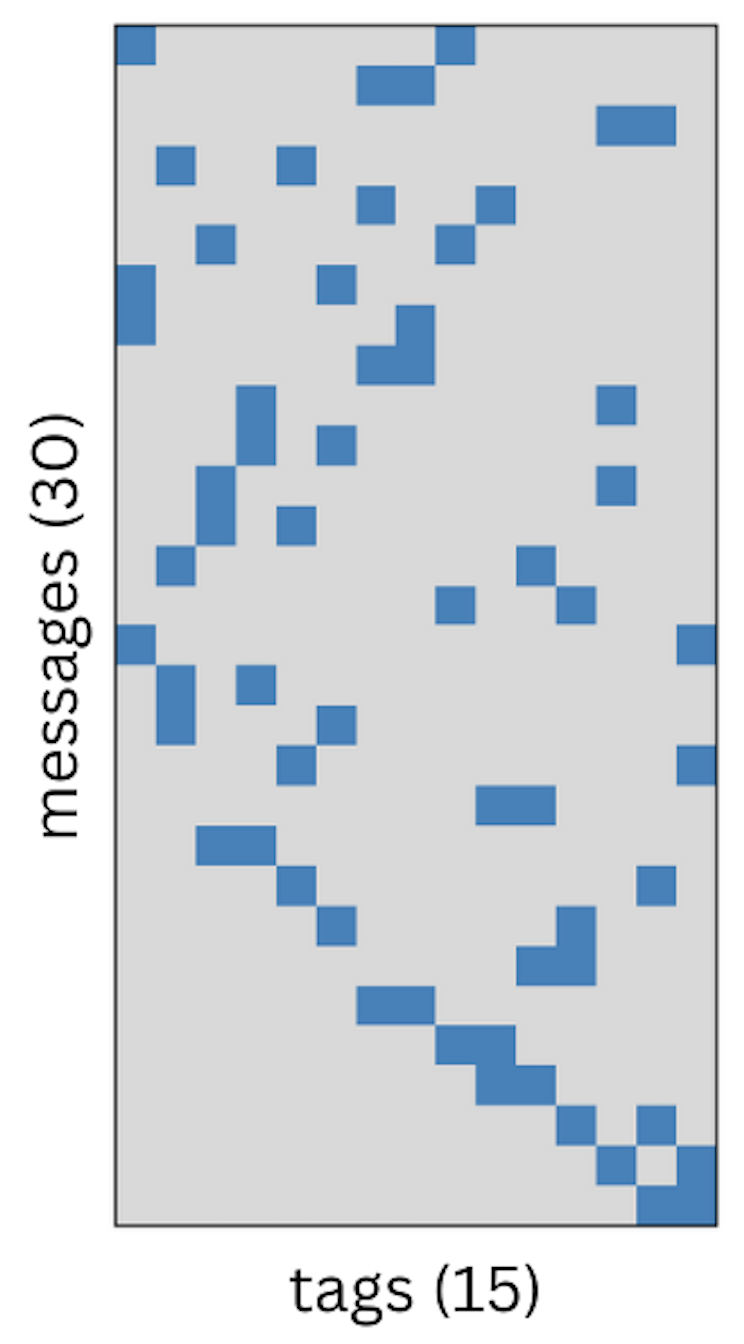
\includegraphics[width=0.38\columnwidth]{img/X.png}
%     \caption{An optimized $X$  matrix of TMR = 15/30.}
%     \label{fig:xmatrix}
% \end{wrapfigure}
 usually depending on the size and the number of tags they generate or transmit per message. However, comparing different schemes' efficiency is difficult, and to simplify comparison, we assume these schemes deploy the same algorithm and generate the same tag size. Based on this assumption, We define TMR ($\frac{n}{m}$), a metric designed to evaluate the efficiency of integrity check schemes, given by:

\begin{equation}
    \frac{n}{m} = \dfrac{\text{total number of tags}}{\text{total number of messages}}
\end{equation}
 
Assuming that transmitting number of tags is less than or equal to the number of messages, $\frac{n}{m}$ provides a normalized value between 0 and 1, where 0 indicates the optimal scenario where no tags are used, representing the highest possible efficiency and 1 indicates that the scheme has no improvement over the traditional method (one tag per message).
\begin{figure}[h]
    \centering
    
\includegraphics[width=.8\linewidth]{img/results/X.png}
    \caption{Two Optimized Matrix \textbf{X} with TMR = 10/25 and 15/25  from left to right, respectability. The yellow squares indicate a 1 representing a message to a tag assignment.}
    \label{fig:placeholder}
\end{figure}





\subsubsection{Tag-bits per Message (TbpM)}
Although Goodput shows the bandwidth efficiency of the MAC schemes, it does not capture the system's security strength. For example, in the Whips shown in Figure~\ref{fig:proMAC}, for every message to achieve a security equal to 258-bit, three tags of size 86 bits are required. However, A packet loss, as shown in equation~\eqref{proMAC_packetLoss_example}, resulted in 9 fewer verifications than expected, equivalent to 774 fewer bits of security overall.

Therefore, we define Tag-bits per Message as follows: 
\begin{equation}\label{tbpm}
    TbpM = \frac{\sum_{i  = 1}^m \sum_{j \in \{j \mid X_{ij} = 1 \} } Pr(U_j=1)|t_j|}{m}
\end{equation}
Assuming that  $|t_j| = |t| \quad \forall j $ we can further simplify the equation above:
\begin{equation}
    TbpM = \frac{|t|\sum_{i  = 1}^m E[A_i]}{m},
\end{equation}
where the tag length is represented by $|t_j|$, and there are in total of $m$ messages.
Equation~\eqref{tbpm}, is the expected number of usable tag bits per message for statistical analysis, however for deterministic analysis , the $Pr(U_j=1)$ must be replaced by $U_j$.

\subsubsection{Authentication Latency (L)}
Packet latency is when a packet is sent and when the integrity check scheme verifies it. Multiple factors influence it, including implementation details, data rates, and computational power. Additionally, the latency can vary depending on the network layer where the integrity check is deployed. Our objective is to specifically assess the impact of the integrity check scheme on latency compared to traditional MACs under both ideal and attack scenarios. It's important to note that underlying layers—such as the physical, data link, and transport layers—can also contribute to latency, especially when the system is under attack.

To facilitate a relative comparison with traditional MACs, we assume that all tags and messages are correctly received. Under this assumption, authentication latency is the number of additional messages that must be received before a specific message can be authenticated, assuming messages are transmitted sequentially. For instance, if tag $t_j$ verifies messages \( m_{i+1}, m_{i+3}, m_{i+7} \) then \( m_{i+1}\) can be verified only after \( m_{i+\{2,\cdots,7\}} \) are received, which by our definition, the latency is six.

Let's assume that all the messages are sent in order based on their index. For example, \( m_1 \) is sent first and \( m_2 \) is sent afterward. We define the Tag Maximum Index (\textbf{TMI}) vector, where the \( j \)-th entry is the maximum index of the message that the tag \( t_j \) is verifying.
\begin{equation}
	TMI_j= \max_{i \in \{i \mid X_{ij} = 1\}} i 
\end{equation}

For example, in the compound MAC shown in Fig.~\ref{fig:compoundMAC}, \( TMI_{j+2} \) corresponding to tag \( t_{j+2} \) equals \( i+6 \), since the the messages that are verified by tag \( t_{j+2} \) are \( m_{i+4}, m_{i+5}, \text{ and } m_{i+6}\).
The authentication latency vector \( \textbf{L} \) is defined as follows:
\begin{equation}
	L_i = 
	\begin{cases} 
		\left(\min_{j \in \{j \mid X_{ij}=1 \}} TMI_j \right)-i & \text{if } A_i > 0 \\
		\text{penalty} & \text{otherwise}
	\end{cases}
\end{equation}
The penalty is the value assigned if message \( m_i \) is not verified by any tag. For example, the latency vector for the Progressive MAC is all zeros. However, the latency vector for the Compound MAC will be as follows:
$$L = [2, 1, 0, 2, 1, 0, \cdots]$$

\subsubsection{Strength Number (SN)}
The Strength number SN represents the smallest ratio of messages or tags that, if lost, would prevent the verification of all messages. An upper bound for the strength number is the total number of tags divided by the number of messages, as destroying all tags would result in no verifiable message. If the set consists only of tags, it must include all tags to ensure no message can be verified. However, any tag within this set can be replaced by a message it verifies. If tag-to-message substitutions are selected strategically in a way that for at least two tags, a common message is replaced, the resulting set can potentially have a cardinality less than the number of tags.

Thus, the strength number can be formulated as the minimum number of messages that will make all the tags unusable divided by the number of messages. As a result, let \( \textbf{S} \subseteq \{m_1, m_2, \ldots, m_m\} \) and for any tag, there exists a message in SN that is verified by that tag. 
\begin{equation}
	\textbf{S} = \left\{m_i \mid \quad \forall j, \exists i \quad \text{such that} \quad X_{ij}=1 \right\} 
\end{equation}
The $|\textbf{S}|$ must be minimized to find the strength number. 
% This can be achieved by finding the minimum set of rows in the \( X \) matrix that, when summed, produces a row with all elements greater than or equal to one. To compare different schemes, \( |\textbf{S}| \) can be divided by the total number of messages \( |M| \) to be normalized.
For a given matrix $X$, finding the strength number is similar to the classical set covering the problem with the following formulation. We define a binary variable \( s_i \) for each message.
\begin{equation}
	s_i =
	\begin{cases} 
		1 & \text{if message $i$ is selected} , \\
		0 & \text{otherwise}.
	\end{cases}
\end{equation}
The mathematical formulation of this set covering problem will be as follows:
\begin{align}
	& \text{min} \sum_{i=1}^{m} s_i  &&  \\
	& \text{subject to}&& \nonumber\\
	& && \sum_{i \in \{i| X_{ij}=1\}} s_i \geq 1, \quad \forall j \in \{1, 2, \ldots, n\} \label{setCoveringConstraint} \\
	& && s_i \in \{0, 1\}, \quad \forall i \in \{1, 2, \ldots, m\}
\end{align}
In this formulation, the constraint~\eqref{setCoveringConstraint} guarantees no message will be verified. The objective function is of type cardinality, effectively counting the minimum possible number of messages that guarantee the total failure of the system. Note that the constraint~\eqref{setCoveringConstraint} should only be used for the active tags in $X$.  Further, $|S|$ must be normalized by the number of messages. Therefore $SN$ is given by:
\begin{equation}
	SN = \dfrac{\text{min}(|S|)}{m},
\end{equation}
where $m$ is the number of messages. The strength number effectively measures the security in terms of availability, representing the percentage of packet loss that results in system failure.
\begin{figure}[h]
	\centering
	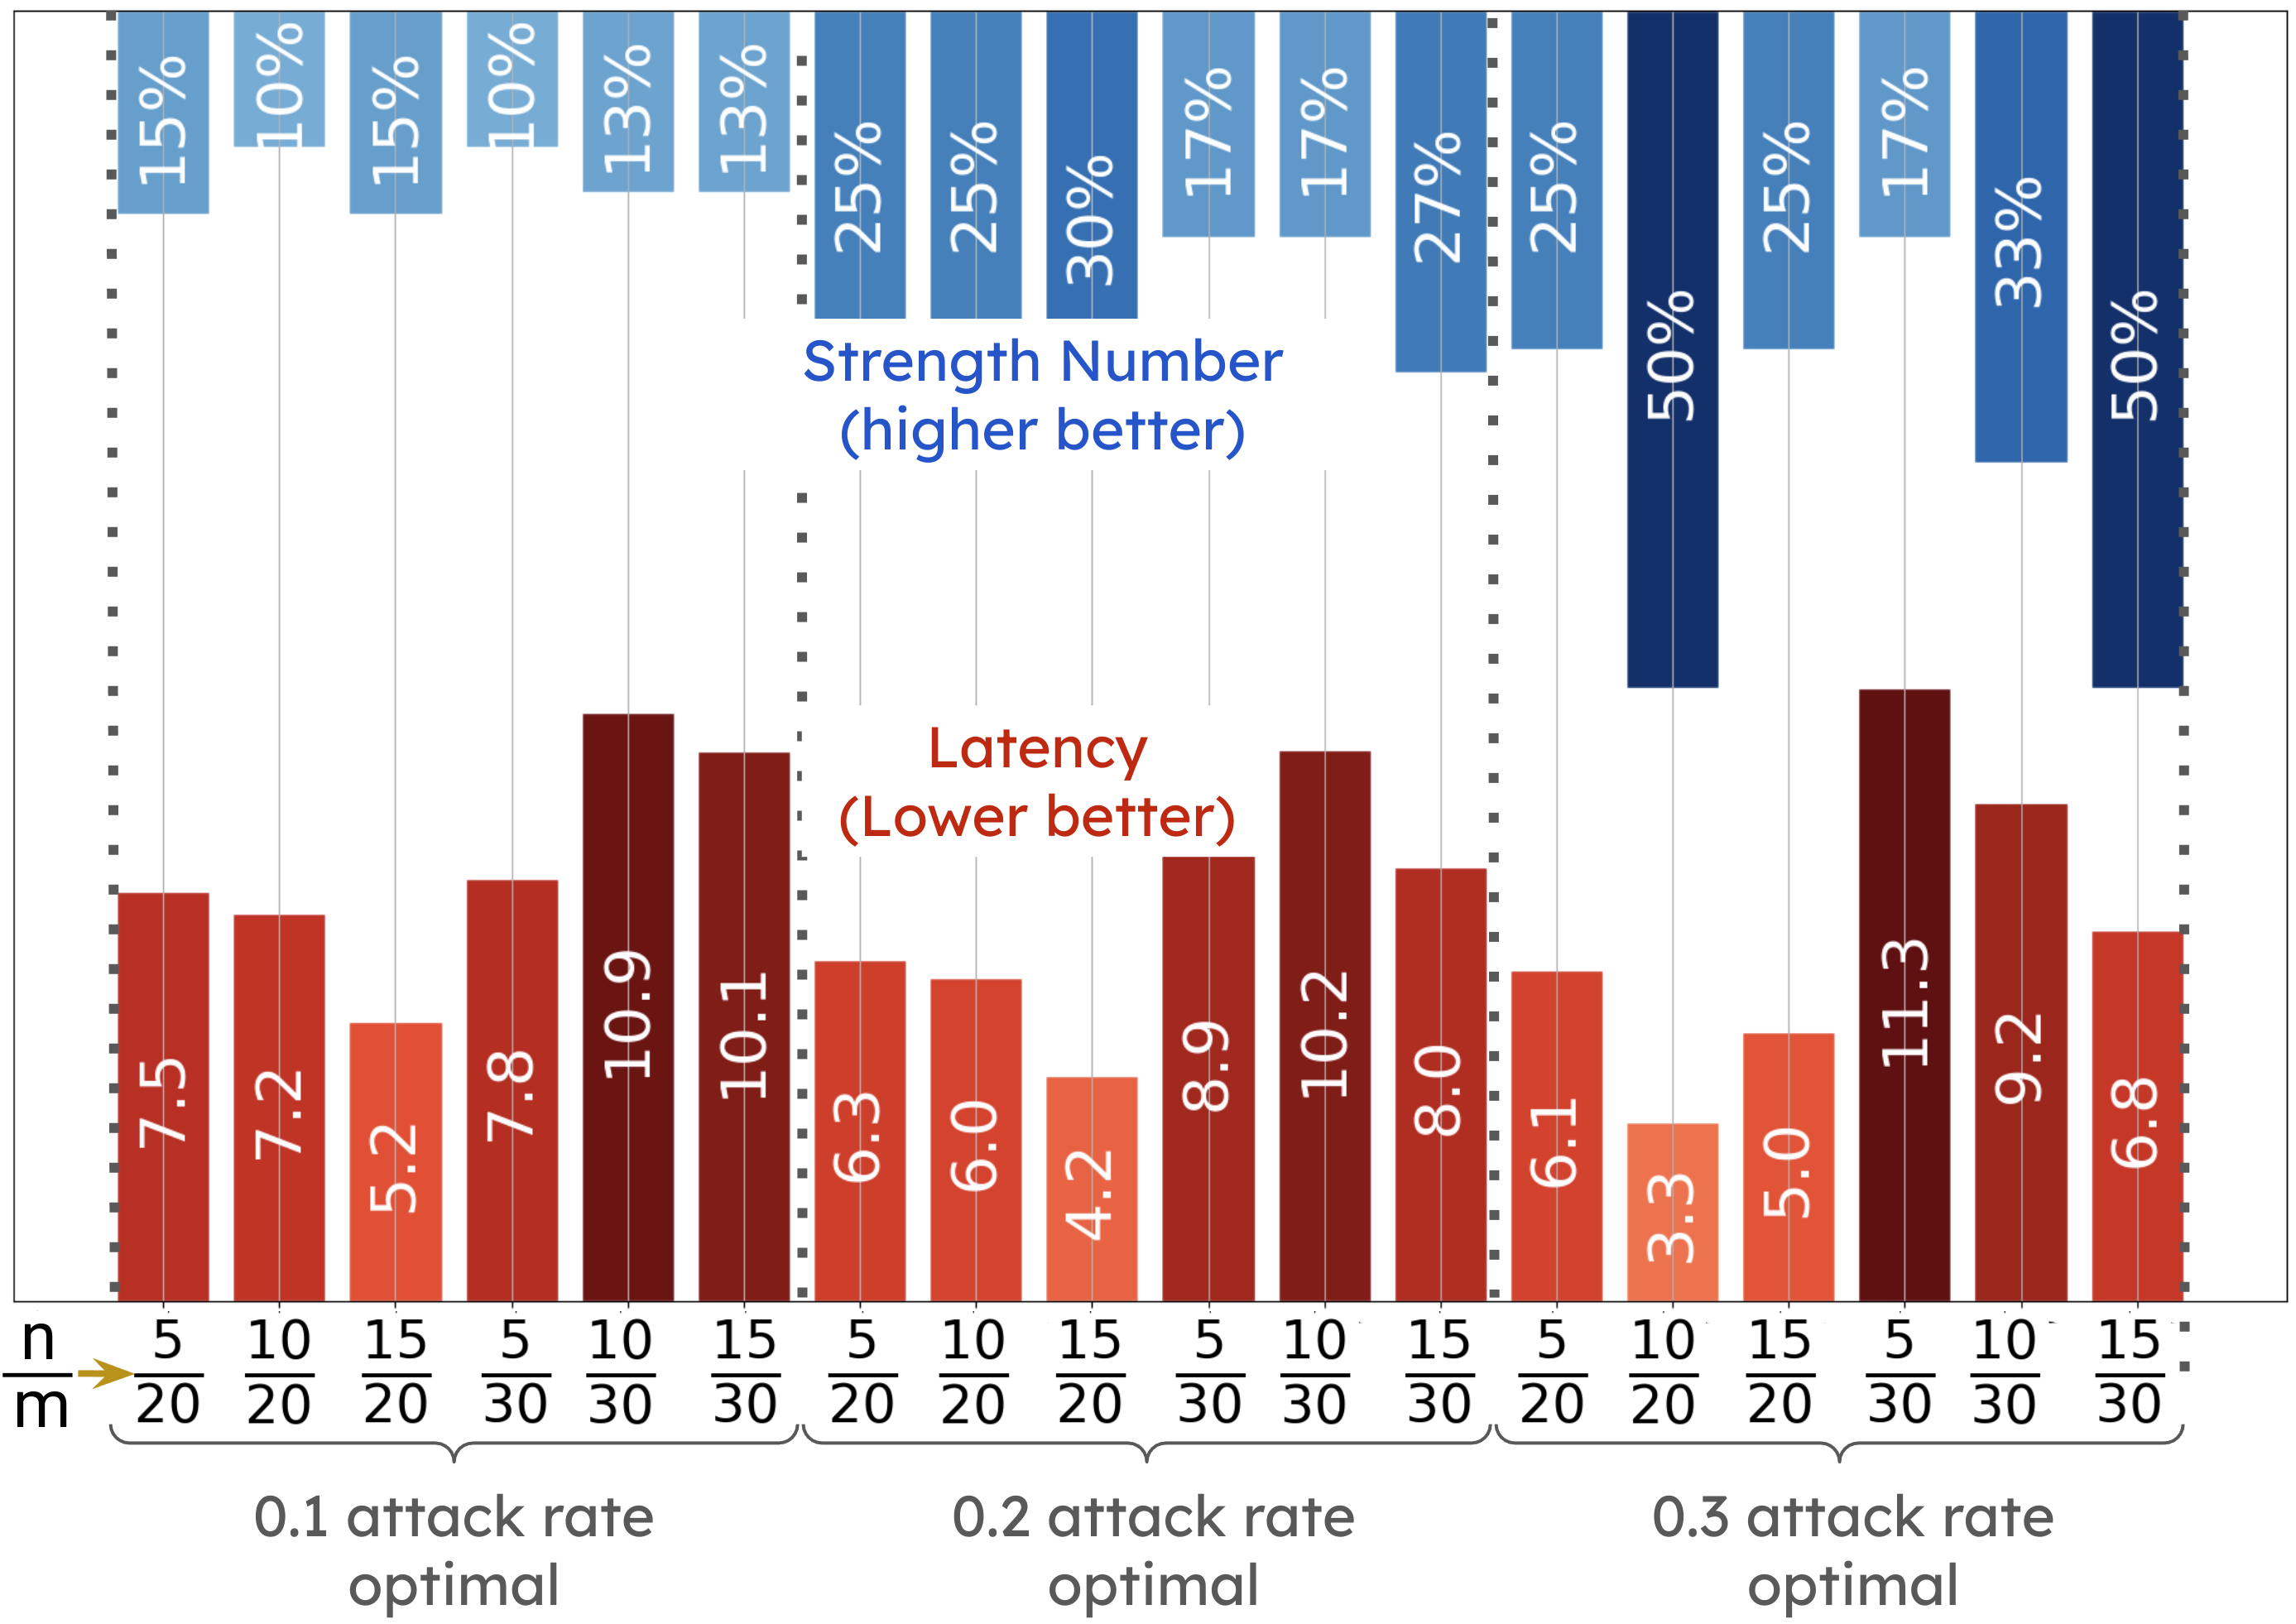
\includegraphics[width=.9\columnwidth]{img/results/SN vs Latency.png}
	\caption{Strength Number and Latency for the optimal solution by attack rates and Tag-to-Message Ratio ($\frac{n}{m}$).}
	\label{fig:otehrMetrics}
\end{figure}
Figure~\ref{fig:otehrMetrics} provides a comparative analysis of the effects of the optimization model on Strength Number (SN) and Latency (L) across different configurations optimized for three distinct attack rates: 0.1, 0.2, and 0.3. Each section corresponds to a specific attack rate and displays bars representing the values of SN (in blue) and L (in red) for various schemes, where each scheme is characterized by a different TMR \( n/m \).


%\subsection{Simulation under Periodic Jamming}
%
%We simulated the transmission of $100{,}000$ packets under periodic jamming,
%where every other message is dropped with probability $p$. Each packet carries
%a $32$-bit message, and the tag sizes were optimized to satisfy a $256$-bit
%security requirement. Figure~\ref{fig:periodic} illustrate the goodput of prior scheme compared to OptiMAC.
%\begin{figure*}
%	\centering
%	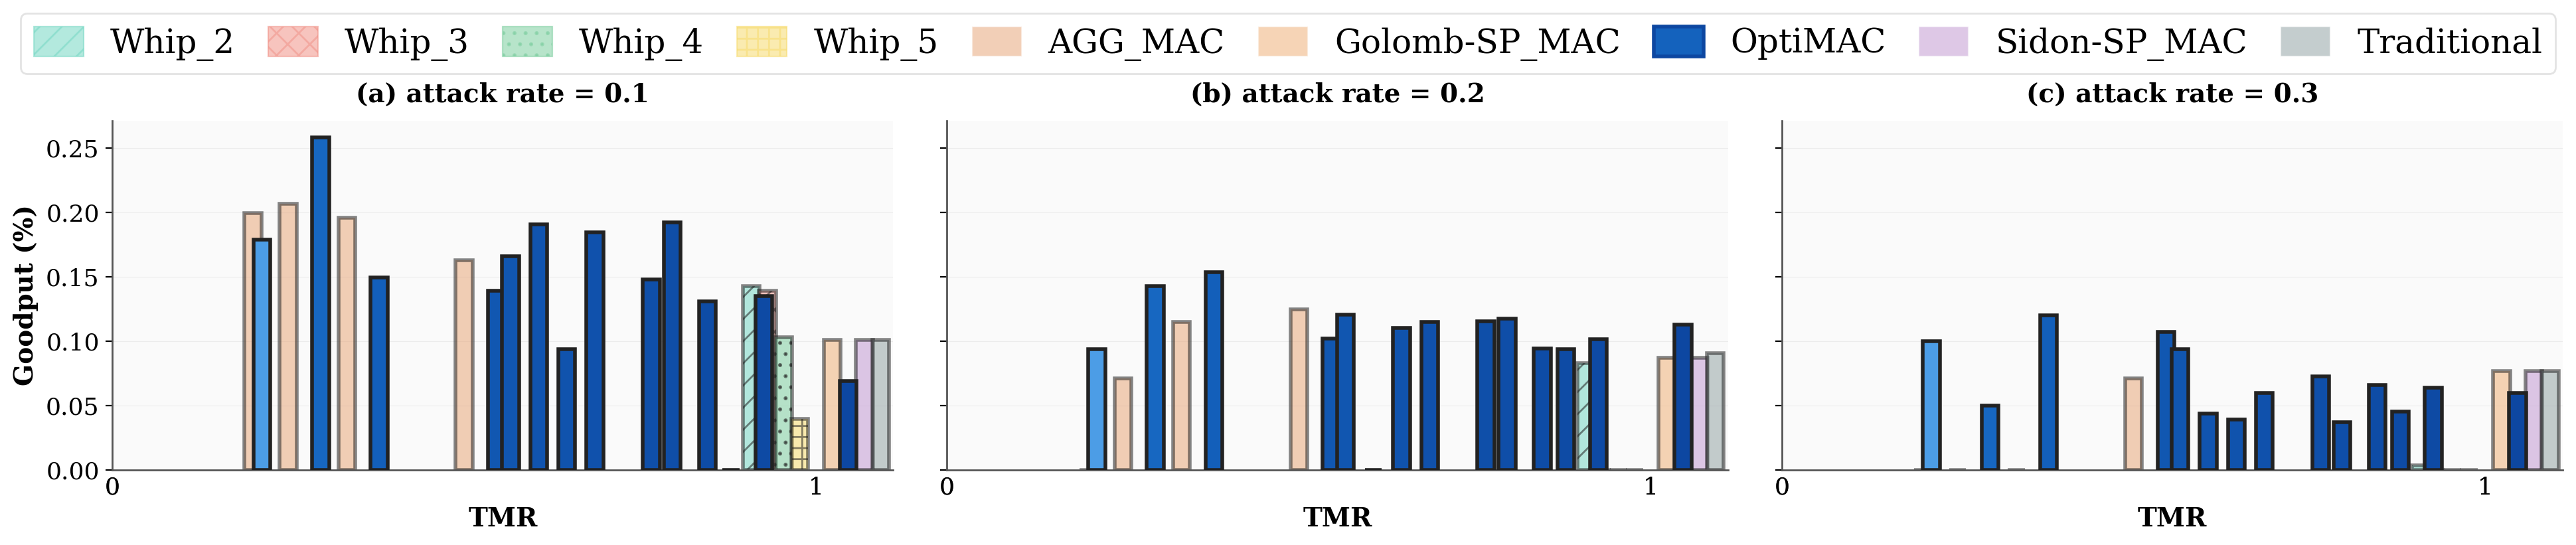
\includegraphics[width=.95\linewidth]{img/output2.png}
%	\caption{Periodic jamming simulation for message size of 32 bits and security requirements of 256 bits. OptiMAC is the only scheme that can provide adaptive solutions for TMR between 1/2 and 1.}
%	\label{fig:periodic}
%\end{figure*}
%
%The results highlight several key observations. First, most prior schemes are
%restricted to a TMR of exactly one (Traditional, WHIP variants, ...), meaning that every message must be accompanied by a tag. aggregate MAC partially relaxes this by offering ratios of $1/n$, but still only at fixed discrete points. By contrast, OptiMAC supports \emph{arbitrary} TMR values, enabling a much finer adjustment between security and throughput. This flexibility translates into higher goodput across a wide range of $p$ values, particularly under severe jamming conditions ($p=0.6,0.7$), where OptiMAC consistently achieves the best
%performance among all schemes.



\subsection{Real-world Testbed}
We have created two real-world testbeds to evaluate the impact of packet interference on webcam video streaming using the UDP protocol on WiFi and 5G networks. The interference sources included an attacker modifying packet data. The objective is to assess the impact on transmission integrity and performance metrics, particularly under adverse conditions.

\subsubsection{WiFi Testbed Setup}
The experimental setup involved a host machine connected to a Logitech HD Pro C920 X webcam, which captured real-time video frames at a resolution 1080p and a frame rate of 30 fps. These frames were transmitted over a WiFi network using the UDP protocol. The UDP packets were customized by appending additional tags according to matrix \textbf{X}.

The transmitter was equipped with an Intel WiFi 6 AX200 (rev 1a) adapter, configured on a Linux Ubuntu 24.04 LTS system with an Intel Core i7-11700K processor. The WiFi hotspot was managed using the nmcli tool, configured to operate on the 802.11 bg at 2.4 GHz band. The video data was encoded using JPEG Progressive format, with varying quality settings 25\% corresponding to data 650  KB/s rate.

% A WiFi jammer was introduced to the experimental setup to simulate signal interference. The jammer hardware consisted of USRP B210 Software Defined Radios (SDRs) and VERT2450 antennas. The WiFi protocol uses Carrier Sense Multiple Access with Collision Avoidance (CSMA/CA) to avoid packet collisions~\cite{wang2006csma}, which means simple constant jamming is not ideal. Therefore a jammer needs to avoid the WiFi protocol's avoidance mechanism to disrupt the transmission by performing random or periodic jamming. This was achieved using Pulse Width Modulation (PWM), with a PWM setting of 10\%. Moreover, there were two different gain settings for the SDR emulating two different jam-to-signal ratios. At the same time, the PWM determines the proportion of time the jammer is active, enabling it to disrupt the transmission and drop packets effectively. The jammer was activated halfway through the experiment to observe its effects on the transmission metrics. It is worth mentioning that the insider attack in our testbed can easily modify and prevent the packet from being sent without any knowledge about other layers and implementation. 

\subsubsection{5G Testbed Setup}
We set up the 5G testbed using an open-source 5G software stack. We use the User Equipment (UE) and gNodeB implementation from OpenAirInterface \cite{oai} and the 5G Core Network from Open5GS \cite{open5gs}. 

The experiment runs on two host machines. Both machines run Ubuntu 22.04 LTS with Intel Core i9-14900K and 64 GB of memory. Host 1 is equipped with 1 USRP B210 software-defined radio and runs the UE 1. Host 2 is equipped with 2 USRP B210s and runs the gNodeB, UE 2, and the 5G Core.  

In our setup, Host 1 acts as the sender. It captures real-time video frames from a Logitech C930e webcam and sends the UDP packets to UE software. The UE 1 running on the same machine receives the packets, processes them in the 5G stack, and sends the data over-the-air to the gNodeB. The gNodeB in Host 2 receives the data from UE 1 and sends it to the Core Network for routing to UE 2. Then, the Core Network routes the packets from the gNodeB over-the-air to the UE 2. Our receiver listening on UE 2 finally receives the transmitted data frame. 
% \yilu{should I draw a figure?}

% Due to the capacity of these software implementations, we can only achieve [list the packet parameters] \yilu{do we need to mention this?}\moh{I don't think so!}

\subsubsection{Transmission Setup}
The transmitted data was structured at the application layer with a custom frame format. Each frame included a 4-byte sequence number, an 8-byte timestamp, and a variable-length data field. 

\renewcommand{\arraystretch}{1.9}

\begin{table}[h!]
\centering
\caption{Experiment parameters for WiFi and 5G}
\label{tab:setting}
\begin{tabular}{c|c|c|c|}
\cline{2-4}
% & \begin{tabular}[c]{@{}c@{}}Data Rate\\ (KB/S)\end{tabular} 
% & \begin{tabular}[c]{@{}c@{}}Payload Size\\ (Bytes)\end{tabular} 
% & \begin{tabular}[c]{@{}c@{}}Tag length\\ (Bytes)\end{tabular} 

&\begin{tabular}{c}
     Data Rate  \\
     (KB/S) 
\end{tabular}   & 
\begin{tabular}{c}
    Message Size\\ 
    (bits) 
\end{tabular}   & 
\begin{tabular}{c}
    Tag length \\
    (bits)
\end{tabular}
\\ \hline 


\multicolumn{1}{|c|}{\textbf{ 5G}}   & 300  & 768 & 512    \\ \hline
\multicolumn{1}{|c|}{ \textbf{WiFi}} & 600  & 128  & 256   \\ \hline
\end{tabular}
\end{table}

\setlength{\tabcolsep}{1.9pt}




The data was then transmitted using the UDP/IP transport layer, to avoid further influence of the transportation layer. The details of the setup configuration for each setting are as follows. To accommodate flexibility to perform integrity checks for any given matrix \textbf{X}, an increase in the complexity of the implementation was necessary. This complexity arose from the need to manage multiple packets before the integrity check was possible, which was achieved by utilizing a book-like buffer structure. In this structure, each "page" holds a certain number of packets based on matrix \textbf{X} dimensions. Once a page is full, it is processed and then released. Although this approach required a larger buffer and introduced additional complexity, we were able to demonstrate that it was manageable by successfully implementing and testing live video streaming at different data rates both in the WiFi and 5G testbed.

The impact of an attacker modifying packets on video transmission was assessed using several key metrics: the number of bits verified per message ($TbpM$), and goodput ($G$). Accurately measuring latency posed a challenge due to the need for precise synchronization between the two devices; therefore, we acknowledge that the latency measurements was not entirely accurate. However, in the future we will try to incorporate a mechanism to reliably measure the latency.





